\section{Grasshopper Components Usage}

Three components are added in a new tab named \textit{Esri}. The main one, whose purpose is to generate the shapes, materials and cga reports. The second one is used to preview and filter the cga reports. The third one is a simple helper component that unpacks the report into its three attributes. The components and corresponding icons can be seen in figure \ref{fig:gh_all}.

\begin{figure}[h]

    \begin{subfigure}{0.5\textwidth}
        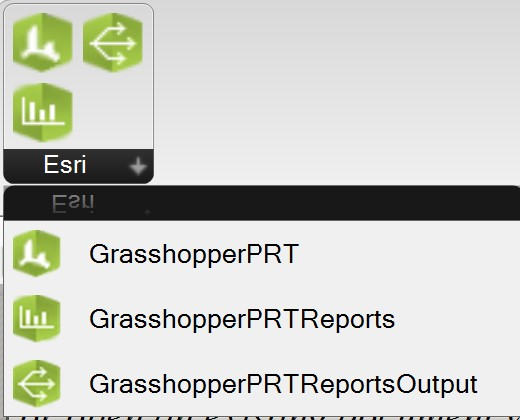
\includegraphics[width=0.9\linewidth, height = 5cm]{res/man_gh_icons.jpg}
        \caption{Icons of the components.}
        \label{fig:gh_subim_icons}
    \end{subfigure}
    \begin{subfigure}{0.5\textwidth}
        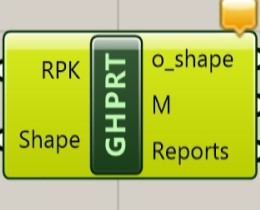
\includegraphics[width=0.9\linewidth, height = 5cm]{res/man_gh_main_comp.jpg}
        \caption{Main component.}
        \label{fig:gh_subim_main}
    \end{subfigure}
    \begin{subfigure}{0.5\textwidth}
        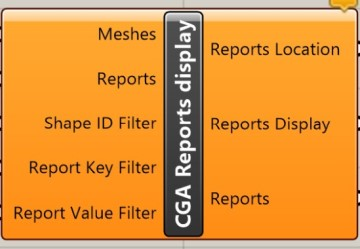
\includegraphics[width=0.9\linewidth, height = 5cm]{res/man_gh_filter_comp.jpg}
        \caption{Report filter component.}
        \label{fig:gh_subim_filter}
    \end{subfigure}
    \begin{subfigure}{0.5\textwidth}
        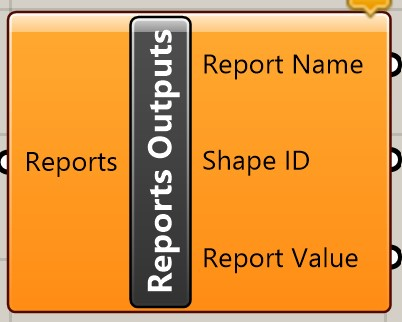
\includegraphics[width=0.9\linewidth, height = 5cm]{res/man_gh_unpack_comp.jpg}
        \caption{Report unpack component.}
        \label{fig:gh_subim_unpack}
    \end{subfigure}
    
    \caption{The Grasshopper components.}
    \label{fig:gh_all}
\end{figure}


\subsection{Main Component}

The main component takes two inputs by default (i.e. Fig \ref{fig:gh_main_input}). The path to a rule package (.rpk), can be provided by connecting a \textit{file path} component. The second input accepts various starting shapes. The list of compatible starting object is as follows: \textit{Mesh, Rectangle, Brep, Surface}.

\vspace{0.1in}

\begin{wrapfigure}{r}{0.5\textwidth}
    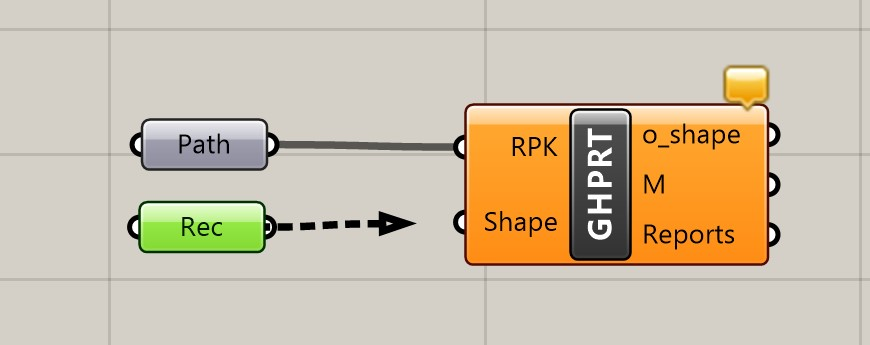
\includegraphics[width=0.9\linewidth]{res/man_gh_init_shape}
    \caption{Main component input parameters.}
    \label{fig:gh_main_input}
\end{wrapfigure}

This implies that any build-in Grasshopper component providing such objects can be connected to this parameter. Figure \ref{fig:gh_main_input} shows how to connect a \textit{Rectangle} component. Figure \ref{fig:gh_set_initial_shapes} shows how to define rectangles: Right-click on the \textit{Rectangle} component, choose \textit{Set one Rectangle} or \textit{Set Multiple Rectangles}. Then, draw the rectangles in the Rhino scene. The way to select shapes can change depending on the Grasshopper component used. The \textit{Surface} component, for example, does not allow to draw a shape, but only to select a previously existing one. It is needed to draw it first using Rhino tools.
\clearpage

\begin{figure}[h]
    
    \begin{subfigure}{0.5\textwidth}
        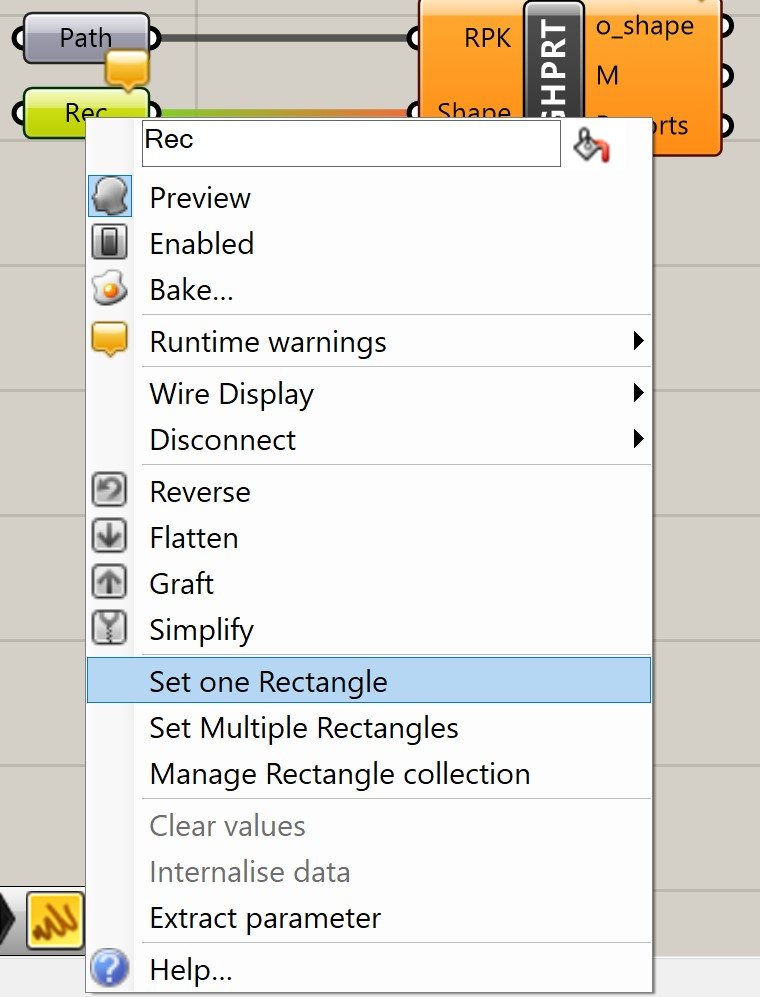
\includegraphics[width=0.9\linewidth, height=7cm]{res/man_gh_select_rectangle.jpg}
        \caption{The option menu of a Rectangle component.}
    \end{subfigure}
    \begin{subfigure}{0.5\textwidth}
        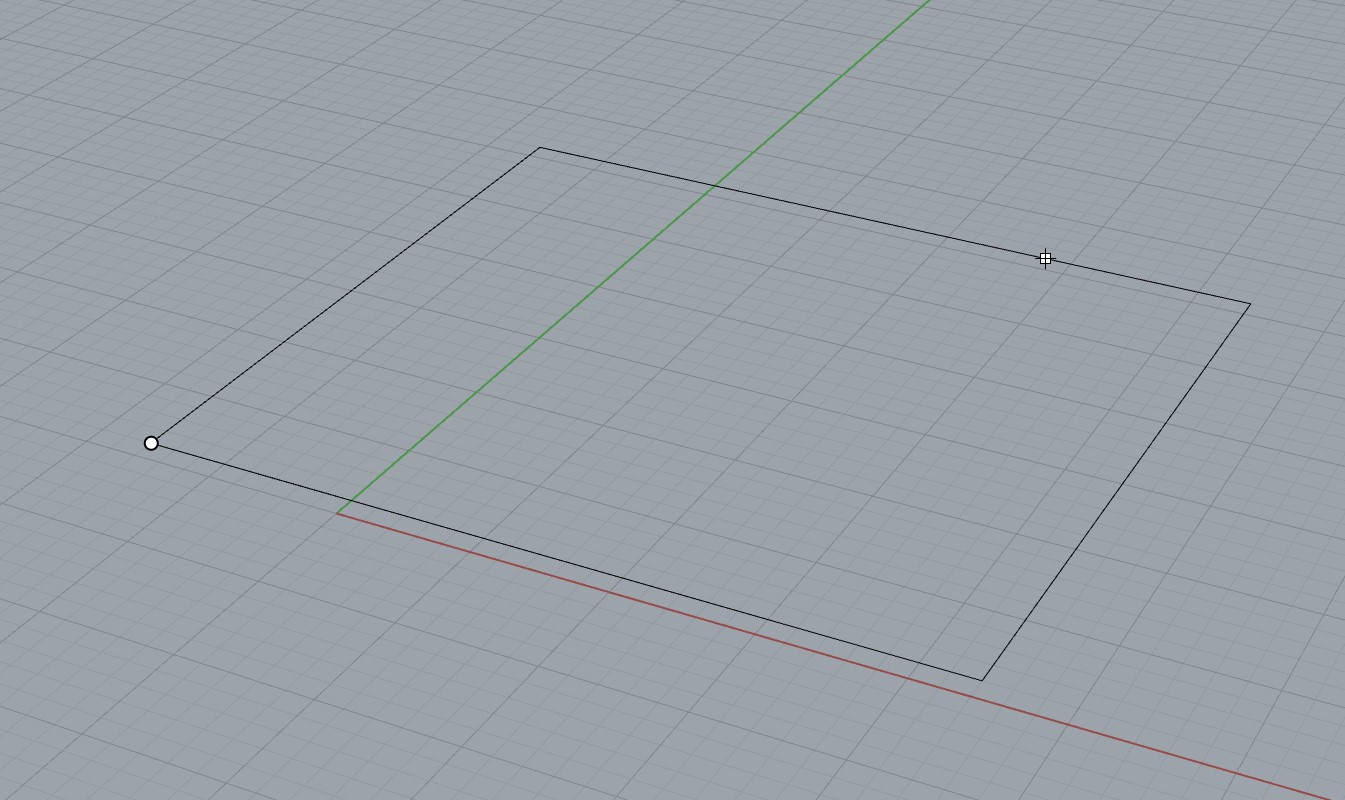
\includegraphics[width=0.9\linewidth, height=7cm]{res/man_gh_select_rectangle_2.jpg}
        \caption{The rectangle is drawn by setting two points.}
    \end{subfigure}
    
    \caption{Set one or more rectangles to use as starting shapes.}
    \label{fig:gh_set_initial_shapes}
\end{figure}

\vspace{0.1in}
When both default inputs are connected, the component is updated with rule attributes defined in the cga rules (Fig \ref{fig:gh_rule_attribs}). These rule attributes are added to the main component as input parameters. These parameters can then be connected normally with other components, or a value can be set directly by right-clicking on each parameter.

\begin{wrapfigure}{r}{0.5\textwidth}
    \centering
    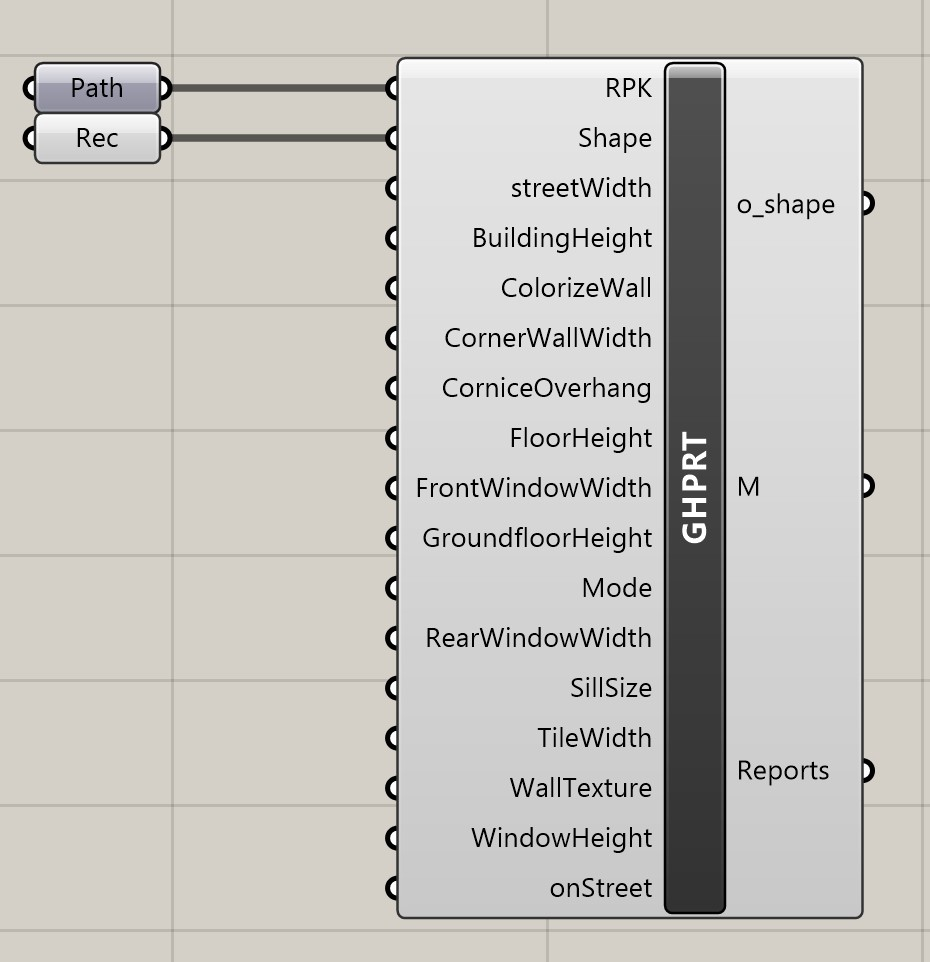
\includegraphics[width=0.9\linewidth]{res/man_gh_rule_attributes}
    \caption{An example of component containing several rule attributes}
    \label{fig:gh_rule_attribs}
\end{wrapfigure}

\vspace{0.1in}
Here is a list of currently supported input parameters and the corresponding components that can be connected to them:
\begin{itemize}
    \item Number (and array of numbers): \textit{number slider}
    \item Boolean (and array of booleans): \textit{Boolean}, \textit{Boolean Toggle}
    \item Text (and array of text): \textit{Panel}, \textit{Text}
    \item Colour (and array of colours): \textit{Colour}, \textit{Colour Picker}
\end{itemize}

In order to gain more information on each rule attribute parameters, the user can hover with the mouse over each of them. A tool-tip is displayed, containing information on the expected data. Figure \ref{fig:gh_tooltips} shows three examples of such tool-tips. Figure \ref{fig:gh_sub_1} is a number parameter that expects a number in the range from 28 to 150. Figure \ref{fig:gh_sub_2} accepts a text parameter. The text can be chosen from a list of accepted choices listed in the tool-tip. Figure \ref{fig:gh_sub_3} shows the tool-tip of a colour attribute with a \textit{colour picker} component connected to it.

\newpage

\begin{figure}[h]
    
    \begin{subfigure}{0.5\textwidth}
        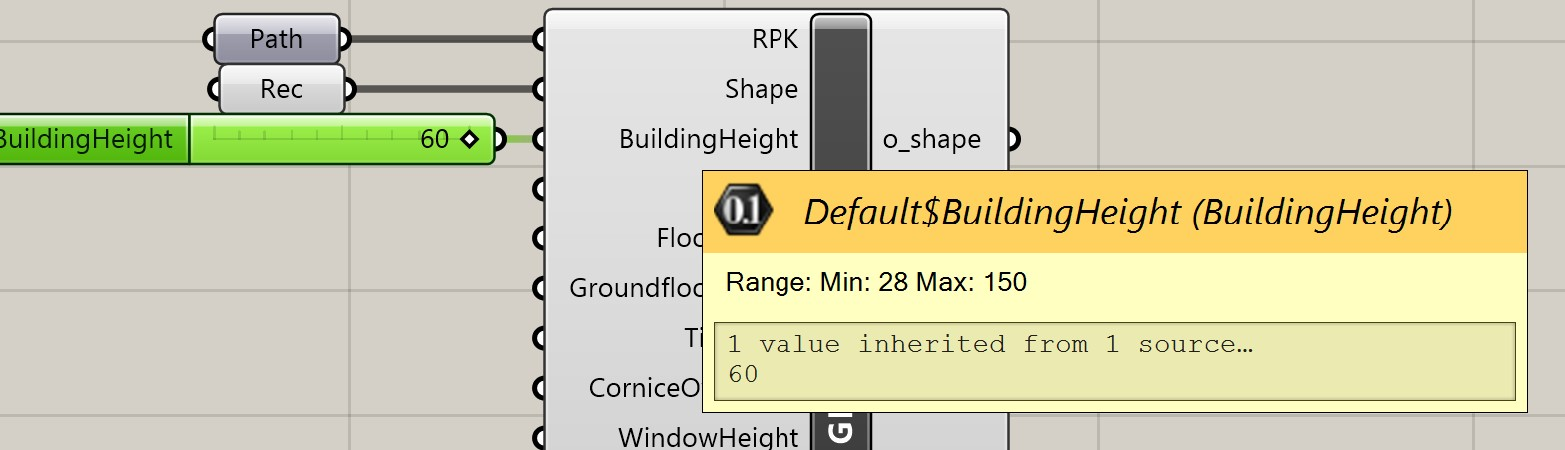
\includegraphics[width=0.9\linewidth]{res/man_gh_input_tooltips.jpg}
        \caption{Tool-tip of a number parameter.}
        \label{fig:gh_sub_1}
    \end{subfigure}
    \begin{subfigure}{0.5\textwidth}
        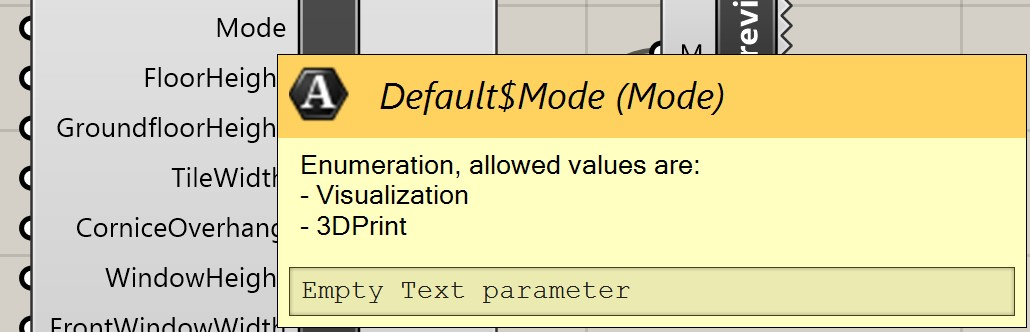
\includegraphics[width=0.9\linewidth]{res/man_gh_enum_tooltip.jpg}
        \caption{Tool-tip of a text parameter accepting\\ list of defined strings.}
        \label{fig:gh_sub_2}
    \end{subfigure}
    \begin{subfigure}{0.5\textwidth}
        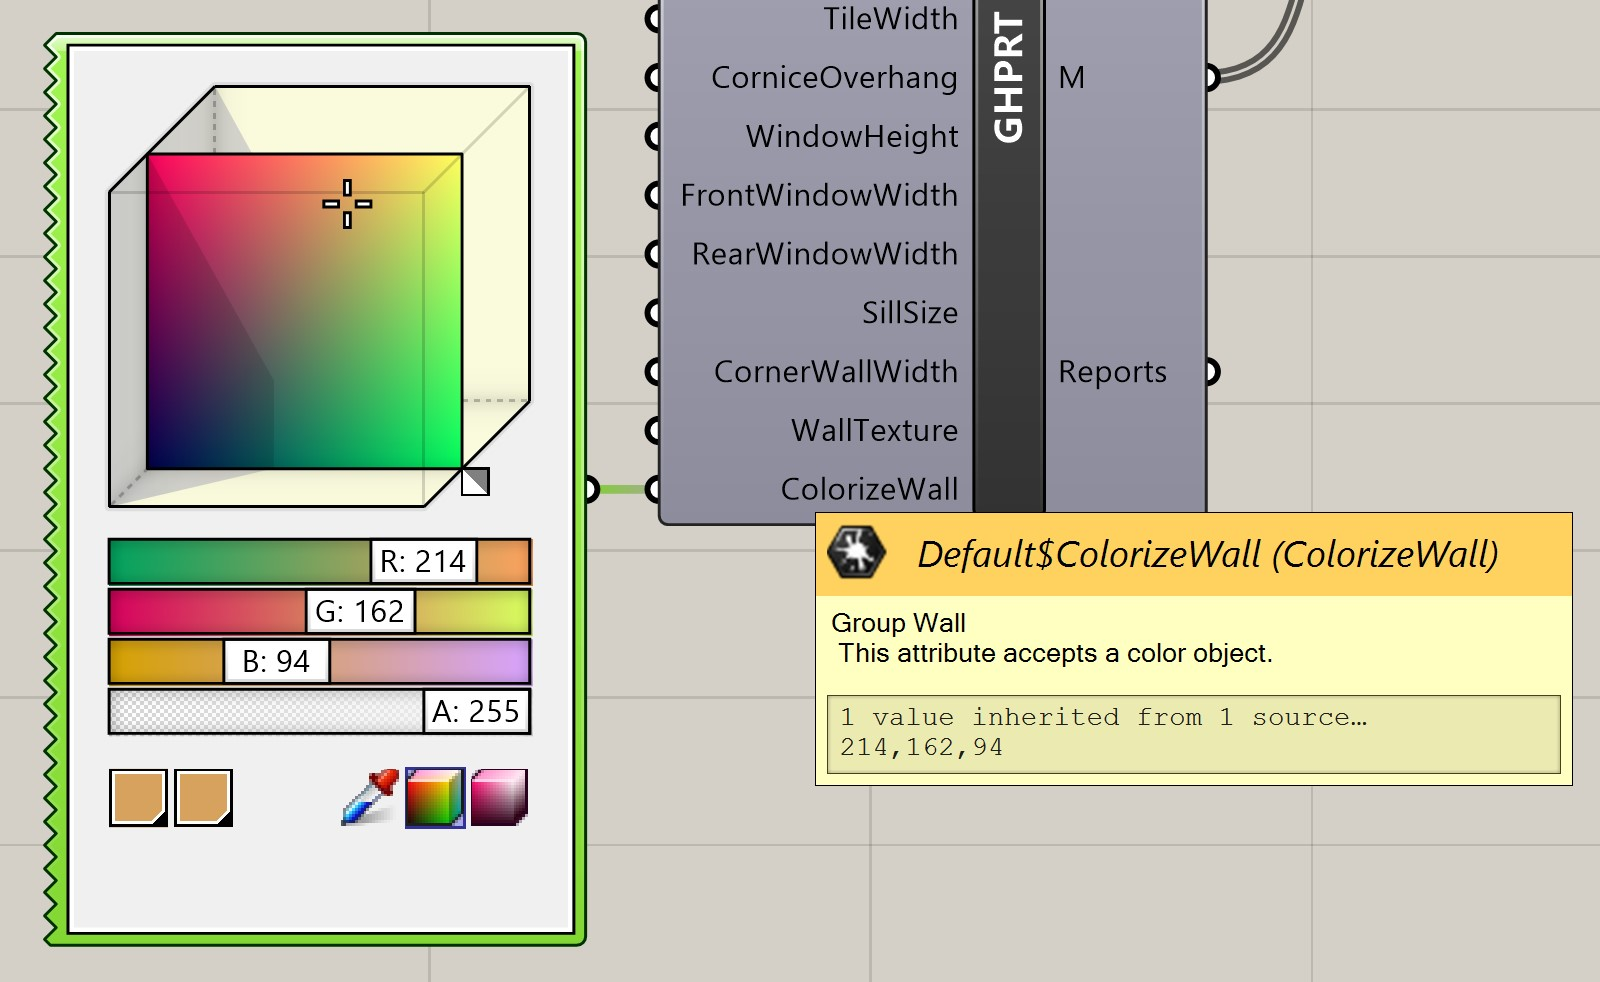
\includegraphics[width=0.9\linewidth]{res/man_gh_color_input.jpg}
        \caption{The color picker component connected\\ to a compatible parameter.}
        \label{fig:gh_sub_3}
    \end{subfigure}
    
    \caption{A few examples of rule attribute tool-tips.}
    \label{fig:gh_tooltips}
\end{figure}

\vspace{0.1in}
It is also possible to right-click on the component and select \textit{Help} to open the \textit{Grasshopper Help} window containing all the necessary information on this component (Fig. \ref{fig:gh_helper}).

\begin{figure}[h]
    
    \begin{subfigure}{0.5\textwidth}
        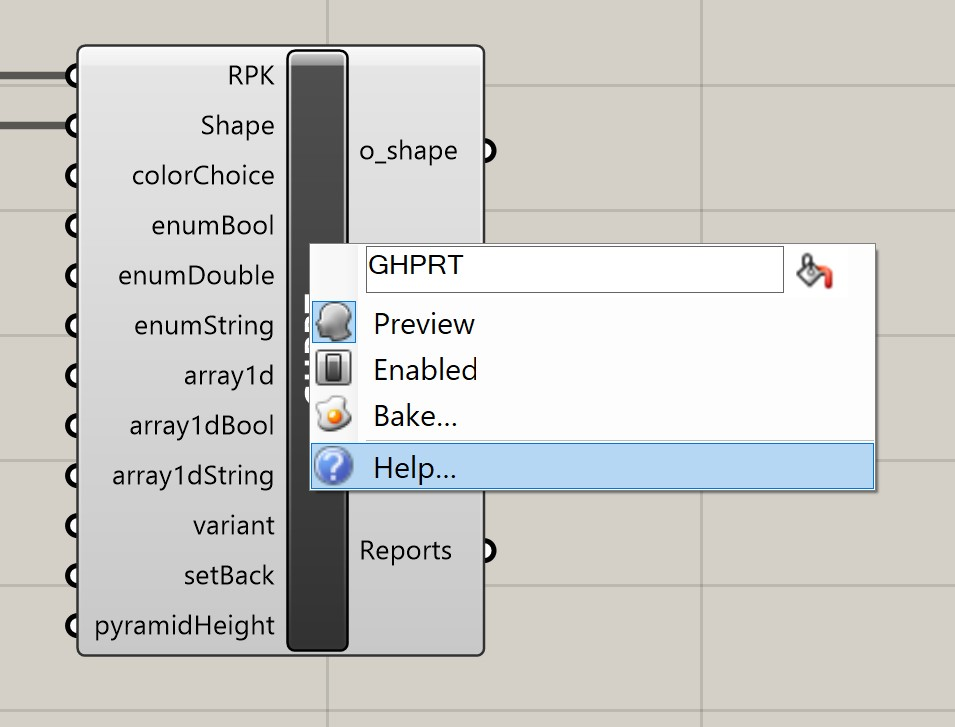
\includegraphics[width=0.9\linewidth, height=6cm]{res/man_gh_helper_0.jpg}
        \caption{Right-clic on the component to open\\ the drop-down menu.}
    \end{subfigure}
    \begin{subfigure}{0.5\textwidth}
        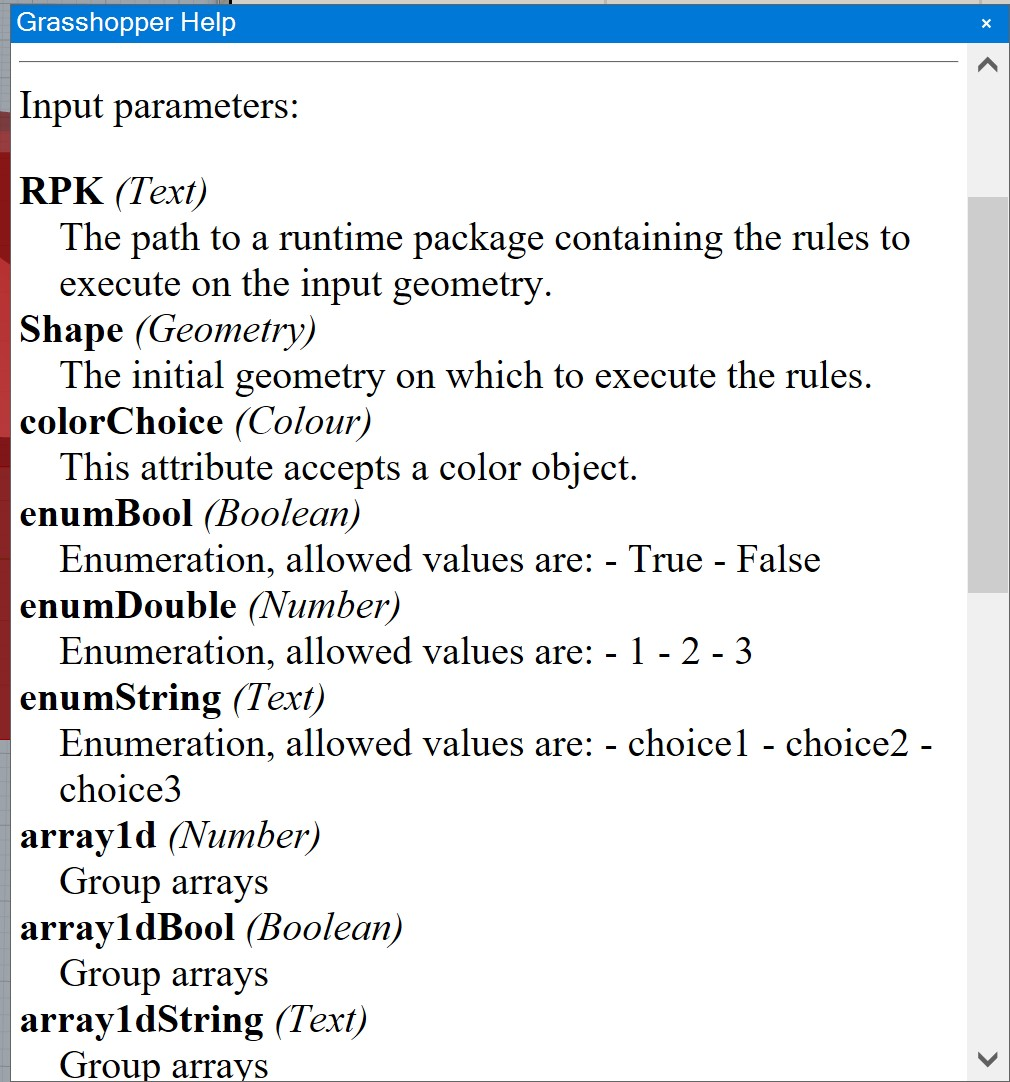
\includegraphics[width=0.9\linewidth, height=6cm]{res/man_gh_helper_1.jpg}\caption{The helper window.}
    \end{subfigure}

    \caption{How to open the helper window.}
    \label{fig:gh_helper}
\end{figure}

\newpage

This component has three outputs:
\begin{enumerate}
    \item o$\_$shape: The generated meshes.
    \item M: The generated materials
    \item Reports: The generated cga reports.
\end{enumerate}

The generated materials can be applied to the mesh by connecting a \textit{Custom Preview} Grasshopper component (Fig \ref{fig:gh_material}). The reports are outputted as a custom type. They are therefore not process-able by built-in Grasshopper components. To address this issue, two helper components are available. They are presented in the next two sections.

\begin{figure}[h]
    
    \begin{subfigure}{0.5\textwidth}
        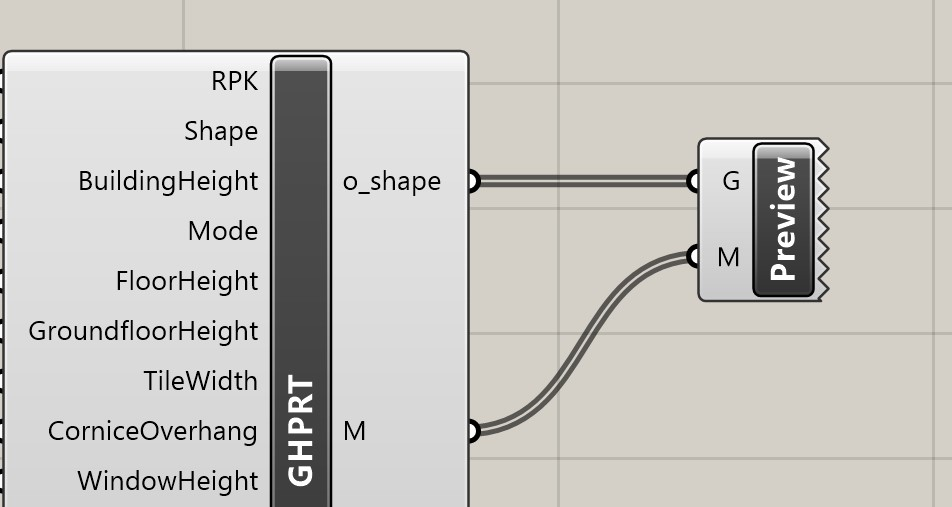
\includegraphics[width=0.9\linewidth]{res/man_gh_apply_material}
        \caption{Use the custom preview component to\\ apply materials.}
    \end{subfigure}
    \begin{subfigure}{0.5\textwidth}
        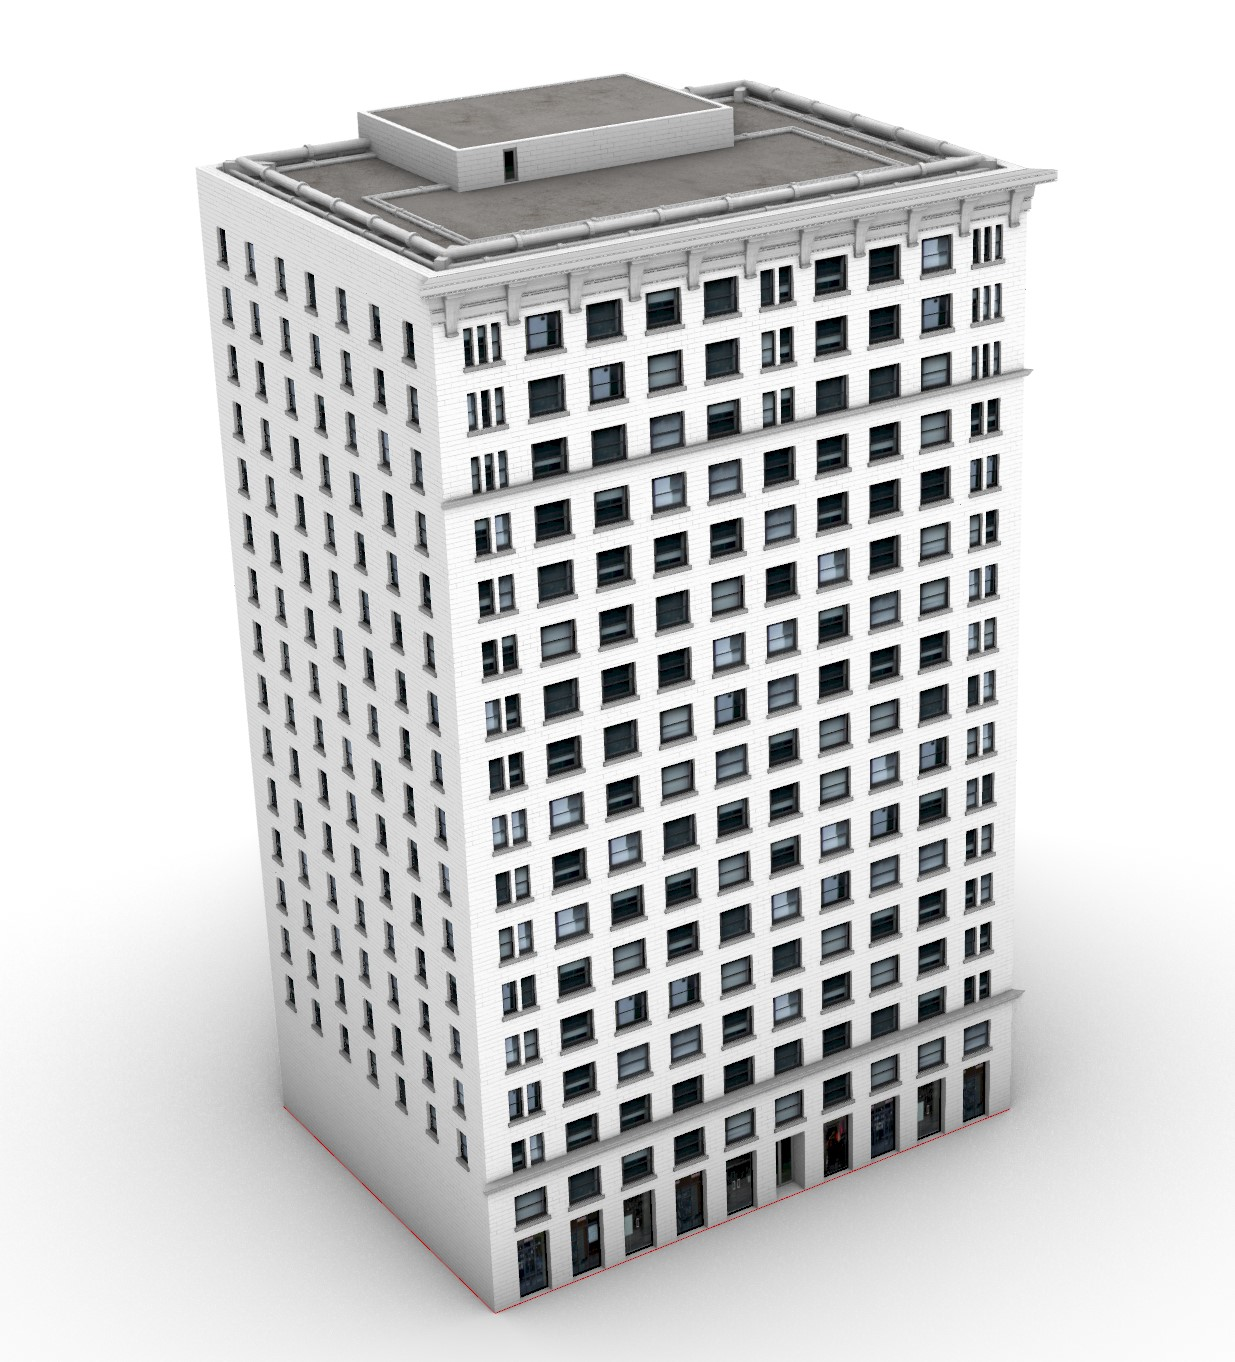
\includegraphics[width=0.9\linewidth]{res/man_gh_candler_result.jpg}
        \caption{An example of material applied to the geometry.}
    \end{subfigure}
        
    \caption{How to apply materials.}
    \label{fig:gh_material}    
\end{figure}

\subsection{Report Filter Component}

\begin{figure}[h]
    \centering
    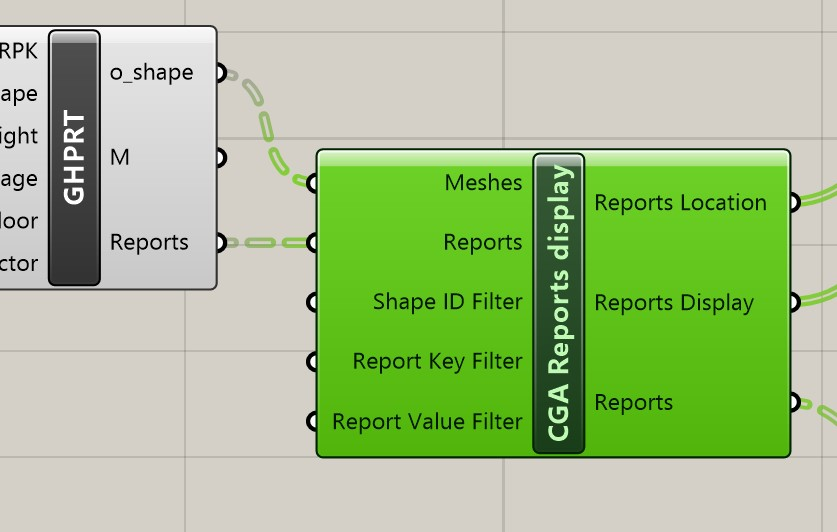
\includegraphics[width=60mm]{res/man_gh_filter_comp_connections.jpg}
    \caption{The report preview/filter component.}
    \label{fig:gh_filter_first}
\end{figure}

This component has 5 inputs. The first two can be connected to the main component's generated meshes and reports as shown in figure \ref{fig:gh_filter_first}. The next three inputs are optional filters:
\begin{enumerate}
    \item Shape ID Filter: Used to filter the reports by initial shape ID. Accepts a \textit{Domain} component.
    \item Report Key Filter: Filters the reports by name. Accepts a \textit{Panel} or \textit{Text} component, or a list of them. Report keys can be written on multiple lines.\\
   \begin{minipage}{\linewidth}
        \centering
        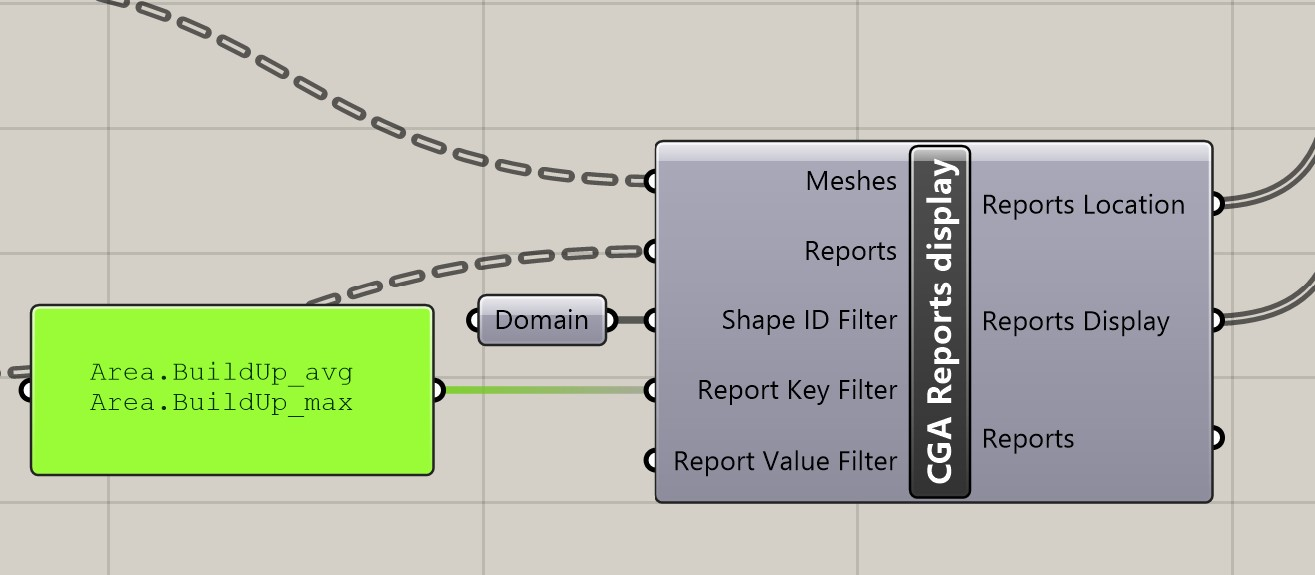
\includegraphics[width=10cm]{res/man_gh_filter_example.jpg}
        \captionof{figure}{Filter value usage.}
    \end{minipage}
    \item Report Value Filter: This input allows to select specific values for each keys selected in the second input.
\end{enumerate}

This component has three outputs, the first two can be connected to a \textit{3D Text Tag} component to display the selected reports in the Rhino view. The first one is simply a located plane used to correctly position and align the reports above each generated geometry. The second one provides the formatted reports, so they can be displayed. The third output simply provides the selected reports. These can then be unpacked by the component presented below.


\subsection{Report Unpack Component}

This helper component is very simple. Its task is to unpack the provided cga reports objects into primitive types that can be further processed by built-in Grasshopper components. It takes as input a list of report objects and outputs, for each report, its name (or key), the initial shape ID it belongs to, and the report value itself. Figure \ref{fig:gh_unpack_example} shows an example of such component.
\vspace{1cm}
\begin{figure}[h]
    \centering
    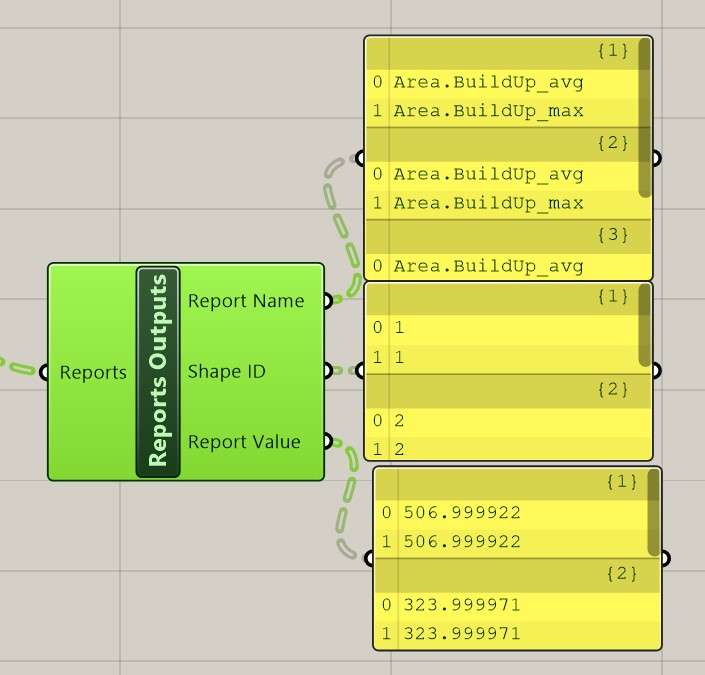
\includegraphics[]{res/man_gh_report_unpack_connected.jpg}
    \caption{Report unpack component.}
    \label{fig:gh_unpack_example}
\end{figure}